\documentclass{article}
\usepackage{titlesec}
\usepackage{graphicx}
\graphicspath{ {./Images/} }
\usepackage{xcolor}
\usepackage{listings}
\usepackage{wrapfig}
\usepackage{subcaption}
\usepackage{float}

\definecolor{mGreen}{rgb}{0,0.6,0}
\definecolor{mGray}{rgb}{0.5,0.5,0.5}
\definecolor{mPurple}{rgb}{0.58,0,0.82}
\definecolor{backgroundColour}{rgb}{0.95,0.95,0.92}

\lstdefinestyle{pythonStyle}{
    backgroundcolor=\color{backgroundColour},   
    commentstyle=\color{mGreen},
    keywordstyle=\color{magenta},
    numberstyle=\tiny\color{mGray},
    stringstyle=\color{mPurple},
    basicstyle=\footnotesize,
    breakatwhitespace=false,         
    breaklines=true,                 
    captionpos=b,                    
    keepspaces=true,                 
    numbers=left,                    
    numbersep=5pt,                  
    showspaces=false,                
    showstringspaces=false,
    showtabs=false,                  
    tabsize=2,
    language=python
}
\author{Juan Alejandro Bernal, Orlando Hernandez}
\title{\textbf{Informe Aplicaci\'on Solucionador De Sudokus}}
\date{\today}

\begin{document}
\maketitle
\section{Problema a resolver}
\subsection{Introducci\'on}
El sudoku es un juego matem\'atico inventado en 1970,  
recibi\'o muy poca atenci\'on del publico en sus inicios, pero en 
la decada de 1984 recibi\'o mucha atenci\'on en jap\'on, finalmente
en el 2005 tomo importancia internacional ya que empezaron
a ser publicados en peri\'odicos.
\subsection{Descripci\'on}
Un sudoku es una cuadricula de 9 x 9  dividida en subcuadrillas
de 3 x 3, en total hay 81 casillas. El objetivo es rellenar las
81 casillas, teniendo en cuenta que algunas casillas ya est\'an rellenadas
de ante mano. La soluci\'on de un sudoku siempre es un cuadrado latino con la \'unica 
diferencia que en cada subcuadrillas no hayan números repetidos.
\subsection{Dificultad}
La dificultad de un sudoku depende del n\'umero de soluciones posibles que hayan 
dependiendo de los valores que est\'an ya dispuestos en las celdas. El matem\'atico Gary
McGuire ha demostrado que el m\'inimo n\'umero de cifras para conseguir un sudoku con una \'unica soluci\'on es de 17 cifras.
Esto se da por que dadas las condiciones del cuadrado latino y que los n\'umeros no se pueden
repetir en subcuadrillas, las posibilidades que existen para poner n\'umeros en lugares equivocados
es muy alta. 
\section{Soluci\'on}
Por la alta dificultad que pueden tener algunos sudokus hemos dise\~nado una aplicaci\'on que se
encarga de recibir un sudoku y devolver una solución.
Haciendo uso de técnicas de reconocimiento de patrones y visión artificial. 
Con la idea de hacerlo m\'as sencillo de usar se creo una aplicaci\'on m\'ovil por medio de Flutter. 
\subsection{Pasos para reproducir la soluci\'on}
\subsubsection{instalacion de Dependencias}
\subsubsection{Manual}
\subsection{Explicación técnica}
En esta secci\'on se describir\'an las t\'ecnicas usadas para construir la aplicaci\'on.
\subsubsection{Visi\'on por computadora}
El algoritmo utilizado para encontrar el contorno de las im\'agenes sigue el contorno binario haciendo
un an\'alisis topologico de la imagen digital, según \cite{test} se sigue un patr\'on de color o intensidad
la cual la computadora sigue como patr\'on de la siguiente manera:
\begin{figure}[H]
\caption{Ejemplo de im\'agenes en visi\'on artificial}
\centering
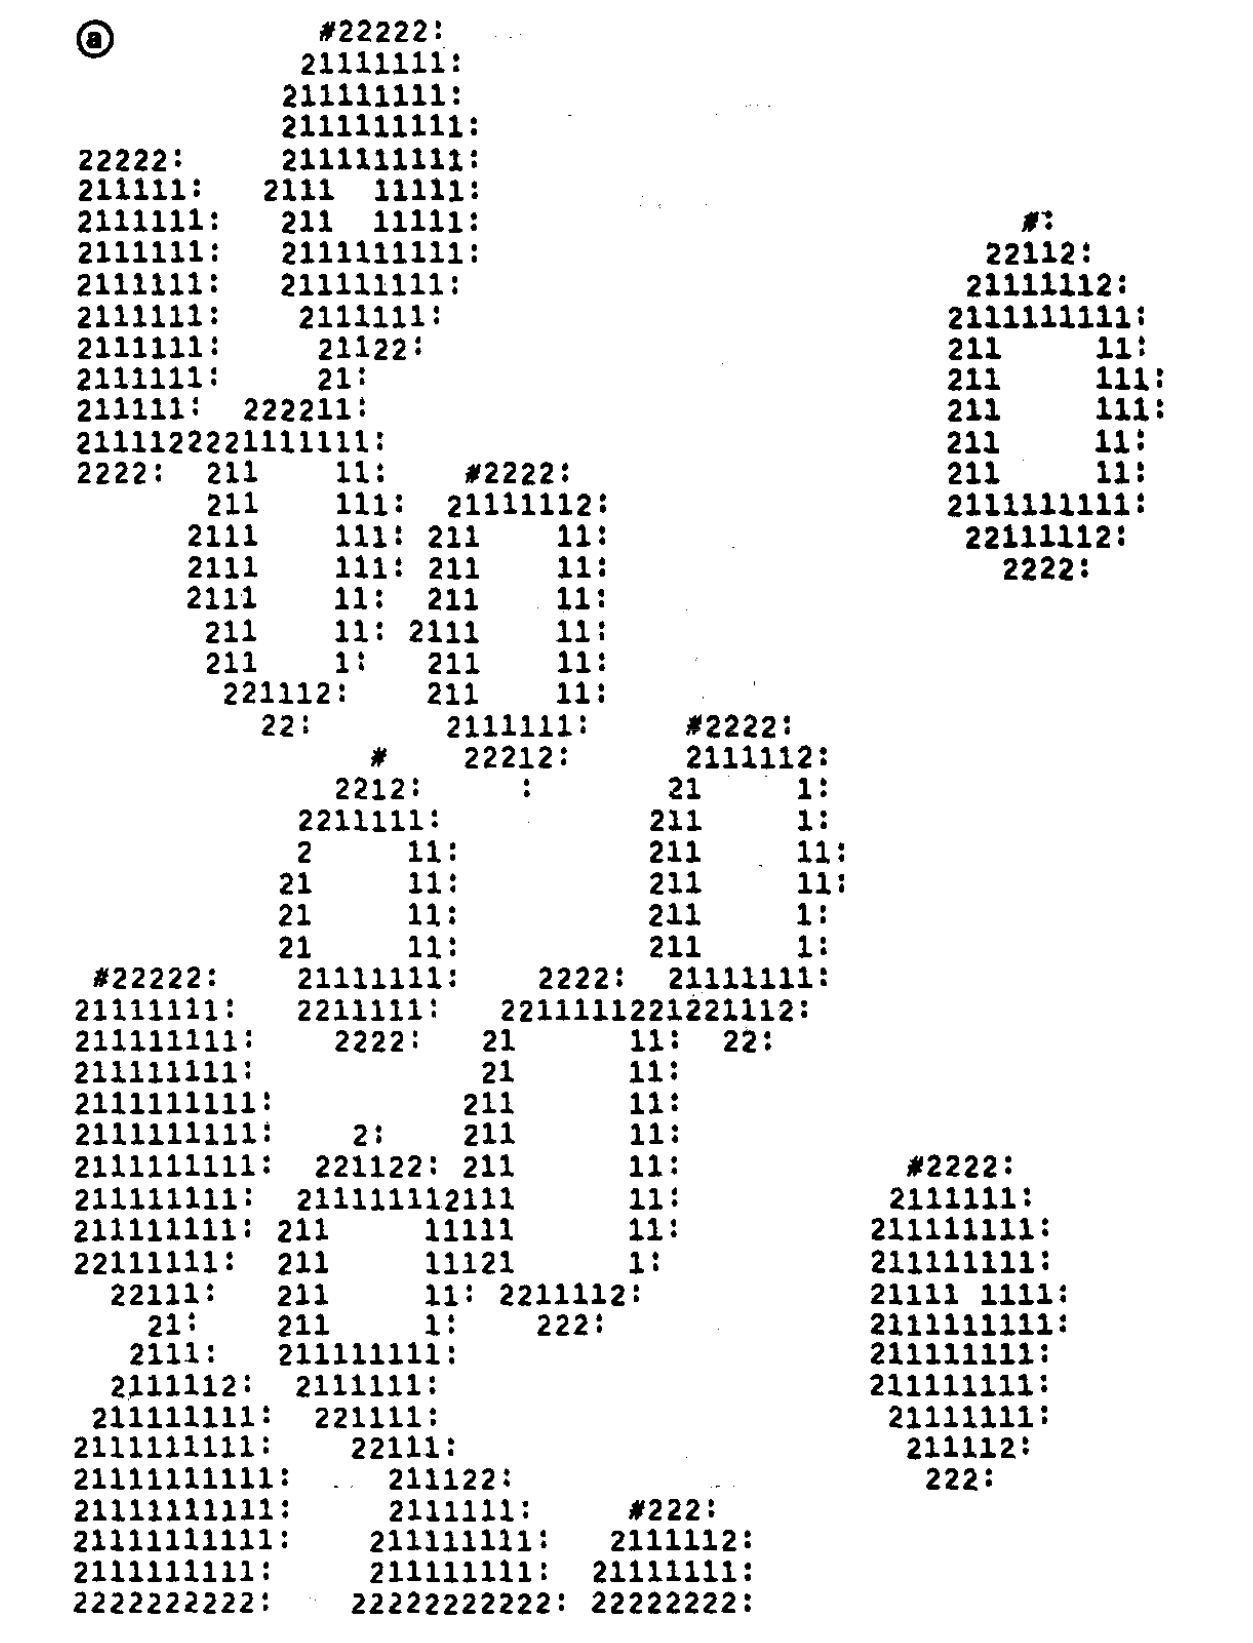
\includegraphics[scale=.15]{a}
\end{figure}
\begin{wrapfigure}{l}{0.4\textwidth}
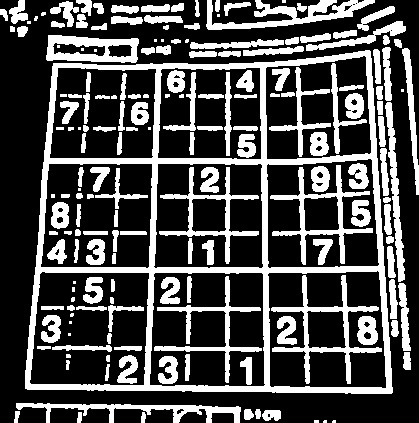
\includegraphics[width=1\linewidth]{filtro}
\caption{Filtro aplicado a un sudoku}
\end{wrapfigure}
Como se puede observar en la imagen los contornos empiezan en el símbolo \# y contin\'uan donde est\'an marcados los
:. El uso de filtros hace que este algoritmo reconozca estos patrones de manera m\'as sencilla, en especial el 
pasar la imagen a un estado binario de forma que quede as\'i:

Haciendo uso de esto podemos conseguir todos los contornos de una imagen de sudoku, al conseguir los contornos
los procesamos haciendo uso del algoritmo de Ramer-Douglas Peucker \cite{ramer} la cual (en resumen) aproxima los puntos
a lineas, las cuales consideraremos como lados, el cual nos permite encontrar todos los cuadrados del sudoku.
Pero como primera instancia debemos de encontrar el cuadrado mas grande, es decir el mas externo.
\vspace{.3cm}
\begin{lstlisting}[style=pythonStyle]
for contour in contours:
         perimeter = cv2.arcLength(contour,True) # largo del contour
         approx = cv2.approxPolyDP(contour, 0.02*perimeter , True) # funcion Ramer, 0.02 es una constante
         if len(approx) == 4: # si es un cuadrado
             if perimeter > maxPerimeter: # para conseguir el contorno mas grande
                 maxPerimeter = perimeter
                 big_square = approx
    return big_square
\end{lstlisting}
Una vez encontrado el contorno m\'as grande nos queda un arreglo con 4 tuplas las cuales representan los puntos
en las esquinas, los cuales usaremos para poder hacer una transformación de perspectiva a la imagen, ya que
como las fotos pueden ser tomadas en \'angulos extra\~nos, se necesita arreglar la perspectiva para que ayude a la
detecci\'on de n\'umeros despu\'es.

\begin{figure}[H]
\centering
\begin{subfigure}{.5\textwidth}
  \centering
  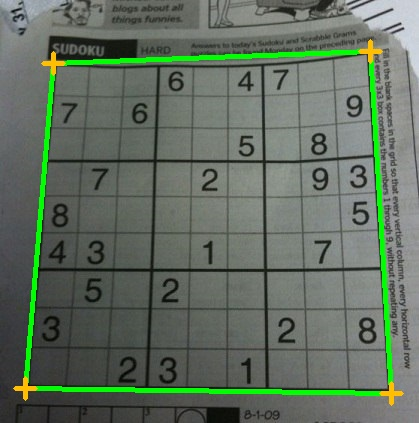
\includegraphics[width=.6\linewidth]{esquinas}
  \caption{Transformaci\'on}
  \label{fig:sub1}
\end{subfigure}%
\begin{subfigure}{.5\textwidth}
  \centering
  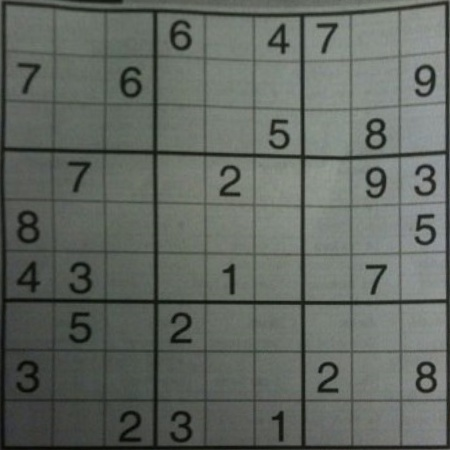
\includegraphics[width=.6\linewidth]{transformada}
  \caption{Esquinas encontradas}
  \label{fig:sub2}
\end{subfigure}
\caption{Procesamiento de imagen}
\label{fig:test}
\end{figure}

Finalmente dividimos el sudoku en sus lineas interiores para poder conseguir
un arreglo de subcuadros, los cuales usaremos para hacer el reconocimiento de 
d\'igitos

\begin{figure}[H]
\caption{Arreglo de subcuadros}
\centering
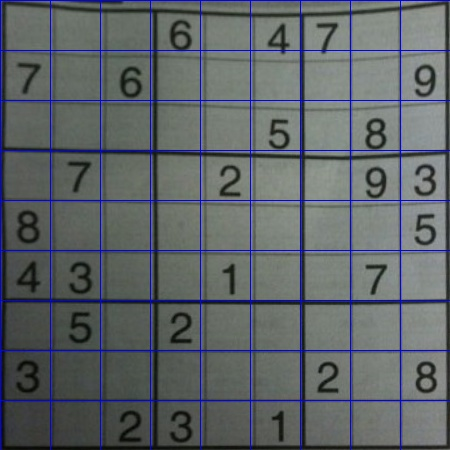
\includegraphics[width=.8\textwidth]{squares}
\end{figure}
% \begin{figure}[h]
% \centering
% \caption{Esquinas de un sudoku}
% 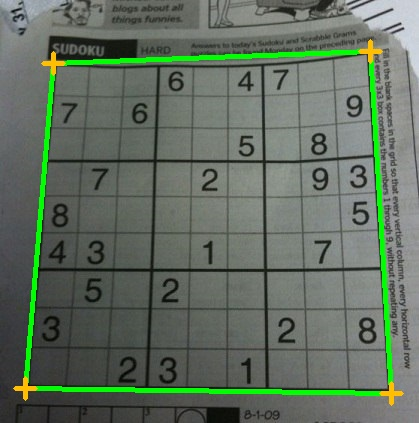
\includegraphics[scale=.3]{esquinas}
% \end{figure}

\subsubsection{Reconocimiento de d\'igitos}
A continuaci\'on, se describir\'a la soluci\'on propuesta para identificar los diferentes n\'umeros encontrados en el tablero del sudoku.
El m\'etodo para la identificaci\'on de los n\'umeros se logra por medio de un modelo que es entrenado por una Red Neuronal Convolucional utilizando el dataset Chars74k. \break
Una red neuronal convolucional es una red que es frecuentemente usada para procesar im\'agenes aprendiendo de relaciones de entrada-salida donde la entrada es una imagen. La operaci\'on b\'asica de una CNN (Red Neuronal Convolucional por sus siglas en ingl\'es) es la convoluci\'on la cual consiste en filtrar una imagen usando una m\'ascara.
\begin{figure}[H]
  \caption{Ejemplo de una convoluci\'on}
  \centering
  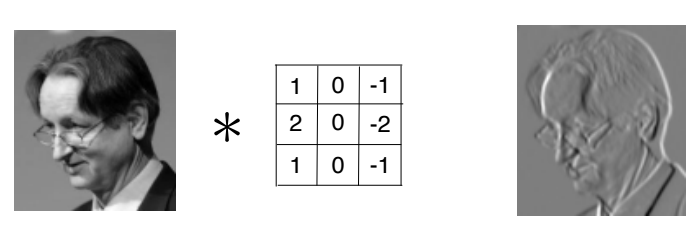
\includegraphics[scale=.50]{convolution}
  \end{figure}

Las 10160 im\'agenes para entrenar a la red fueron tomadas del dataset Chars74K. Estas im\'agenes fueron divididas en el 98\% para el entrenamiento de la red y el restante para realizar la validaci\'on del modelo resultante. Cada una de estas im\'agenes es de fondo negro y contiene un d\'igito del 0 al 9 en color blanco; su tama\~no es de 28x28 pixeles.
\begin{figure}[H]
  \caption{Imagen del dataset Chars74K}
  \centering
  
\includegraphics[]{dtimgexample}
\end{figure}

En 1 se puede observar la arquitectura de la red neuronal propuesta para solucionar el problema.
\begin{figure}[H]
  \caption{Imagen del dataset Chars74K}
  \centering
  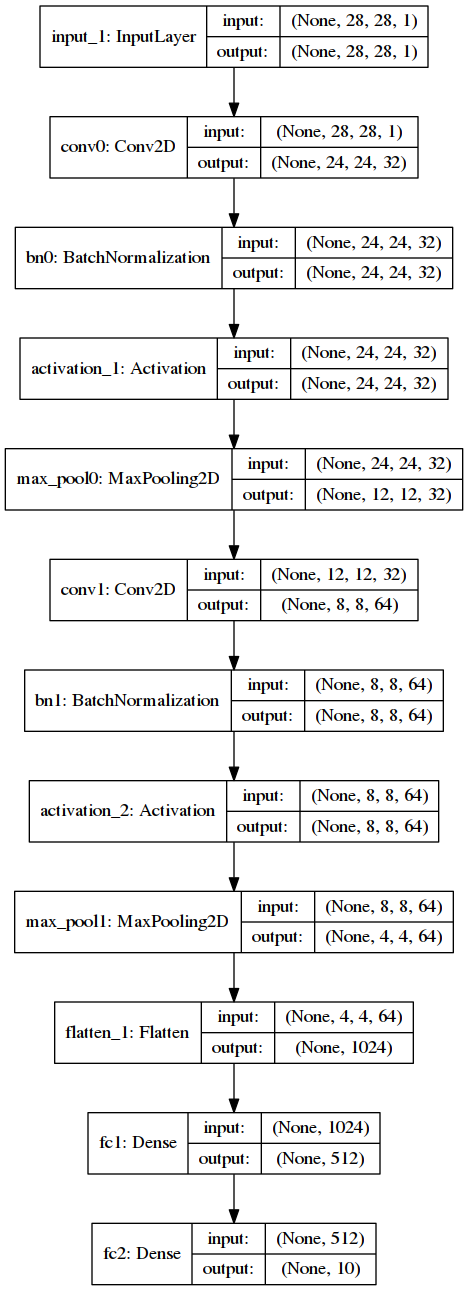
\includegraphics[scale=.40]{model_plot}
\end{figure}
A continuaci\'on, una breve descripci\'on de cada una de las capas:
\begin{itemize}
  \item Una capa convolucional la cual se compone de 32 filtros de taman\~o 5x5 que recorren la imagen con paso de 1
  \item una capa de normalizaci\'on que se encarga de mantener los valoresen el rango...
  \item Una capa que se encarga de ejecutar la funci\'on de activaci\'on reLU la cual se define como se muestra en (1)
  \item Una capa de pooling que se encarga de tomar cada una de las entradas de la capa anterior y reducir su tama\~no
  \item Una capa convolucional la cual se compone de 64 filtros de tama\~no 5x5, estos recorren a cada imagen con paso de 1
  \item De nuevo, una capa de normalizaci\'on
  \item Una capa de que se encarga de ejecutar la funci\'on de activaci\'on reLU
  \item Una capa de pooling con el mismo bjetivo que en el item...
  \item Una capa de aplanamiento
  \item Una capa de una red neuronal simple con 512 neuronas y funci\'on de activaci\'on relu
  \item Una salida con 10 neuronas con funci\'on de activaci\'on softmax definida en (2) que se encarga de devolver la probabilidad de que la imagen tomada como entrada sea de un digito del 0 al 9
\end{itemize}
\subsubsection{Backtracking}
\section{Resultados}
\bibliographystyle{ieeetr}
\bibliography{uni}
    
\end{document}











